\section{波场外推方程}
波场外推方程是一个有关波场之导数(通常是沿深度$z$的方向)的表达式。当已知波场
及其导数时,就可利用$P(z+\Delta z)=P(z)+\Delta zdP/dz$的各种不同数值表示方法来处理外推问
题,所以真正需要的是有关$dP/dz$的表达式。求解$dP/dz$的两种理论方法是早期的变换方法
和较新的波散关系方法。

\subsection{抛物线型波动方程}
在抛物线型方程被引用于石油勘探的时期(1969年),“波动理论不起作用”这种论调
相当流行。在那个时代,石油勘探人员分析地震资料是采用射线方法,波动方程还与实际工
作无缘,唯有大学里的理论家们才会问津波动方程(事实上,波动理论对于比地震勘探尺度
大一千倍的大规模天然地震中的面波,是起过作用的)。即使是大学的研究人员,那时也未
曾完善地建立波动方程的有限差分解,计算机是计算机,解是解,所解决的多为“鼓面振
动”之类的问题,而不是求解“地层中传播的地震波”
。最早是为了提高有限差分波动模拟
的计算效率而才引入抛物线型波动方程,下面对抛物线型波动方程的介绍就是藉助于原来采
用的变换方法。

1969年以前,困难来自于有一个对当时所有地震波理论极为重要而又不恰当的假设,即
水平成层假设。射线追踪曾是摆脱该种假设限制的仅有方法,但采用射线追踪看来就得放弃
地震波形的模拟。在石油勘探中,几乎所有波动理论其本身更进一步还得受垂直入射的限
制。成功地克服困难的途径就在于将垂直入射情形加以推广,沿垂直入射方向周围允许有微
小角度变化范围,放弃许多熟悉但很麻烦的地震理论就达到了这个目的。

垂直下行平面波在数学上以下述方程表示
\begin{equation}
P(t,x,z)=P_0e^{-i\omega (t-z/v)}
\label{eq:ex2.1.1}
\end{equation}
式中,$P_0$纯为常数。将$P_0$用某种不是严格恒定而是缓慢变化的函数$Q(x,z)$来代替,即可
模拟偏离垂直入射的微小角度改变,即
\begin{equation}
P(t,x,z)=Q(x,z)e^{-i\omega (t-z/v)}
\label{eq:ex2.1.2}
\end{equation}
将式\ref{eq:ex2.1.2}代入标量波动方程$P_{xx}+P_{zz}=P_{tt}/v^2$,得
$\frac{\partial^2 Q }{\partial x^2}+(\frac{i\omega}{v}+\frac{\partial}{\partial z})^2Q
=-\frac{\omega^2}{v^2}Q$
即
\begin{equation}
\frac{\partial^2 Q }{\partial x^2}+\frac{2i\omega}{v}\frac{\partial Q}{\partial z}+\frac{\partial^2 Q}
{\partial z^2}=0
\label{eq:ex2.1.3}
\end{equation}
导出此式时,未作任何假设,仅仅是将波动方程用$Q(x,z)$重新加以表示而已。为使波场接近于平面波,$Q(x,z)$
必须接近于一常数。适宜的假设应是$Q$沿深度的最高阶导数、即$Q_{xx}$可忽略不计(首次引入这个假设时,曾引起一些争论),这就使我们得出抛物线型波动方程
\begin{equation}
\frac{\partial Q }{\partial z}=-\frac{v}{2i\omega}\frac{\partial^2 Q }{\partial x^2}
\label{eq:ex2.1.4}
\end{equation}
首次建立这个方程用于地震学的时候,当时认为式\ref{eq:ex2.1.4}的最重要性质是这样一
点:对于接近于沿垂直方向传播之平面波的,一种波场而言,沿$x$轴方向的二阶导数应很小,
因而沿$z$轴方向的导数应很小。所以,应用有限差分方法时将允许采用非常大的步长$\Delta z$,从
而能使处理的模型更像是地层模型而不大像是鼓面。

随后,很快就弄明白了,抛物线型波动方程也正是地震成像方法所需要的那种方程,即
它是一种波场外推方程。

妙极了,式\ref{eq:ex2.1.4}就是量子力学中的Schroedinger方程的形式。

这种办法、即变换方法曾经是而且现在也是非常有用的。不过它很快就为波散方程处理
方法所取代,这是获得以较宽角度进行波场外推的方程的途径。
\subsection{Muir平方根展开方法}
在我们采用较新的求解波场外推算子的方法时,要探索平方根波散关系的各种不同近
似,然后,将近似波散关系反变换为一个偏微分方程。自从我的《地球物理数据处理基础》
一书写成以来,波散关系处理方法已经有了显著进展,这得大大感谢Francis
Muir。

将平面波$exp(-i\omega t+ik_xx+ik_zz)$代入二维标量波动方程,得出波散关系
\begin{equation}
k_x^2+k_z^2=\frac{\omega^2}{v^2}
\label{eq:ex2.1.5}
\end{equation}
求解$k_z$,选择正平方根(选择下行波时即如此)
\begin{subequations}
\begin{equation}
k_z=\frac{\omega}{v}\sqrt{1-\frac{v^2k_x^2}{\omega^2}}
\label{eq:ex2.1.6a}
\end{equation}
为沿$z$轴进行反变换,我们仅需理解相应于反变换所得最终表达式是一个波
场外推算子,即
\begin{equation}
\frac{\partial P}{\partial z}=i\frac{\omega}{v}\sqrt{1-\frac{v^2k_x^2}{\omega^2}}P
\label{eq:ex2.1.6b}
\end{equation}

\end{subequations}
将方程\ref{eq:ex2.1.6b}变换回空间域并非就是用一个有关$x$的二级导数代换$k_x^2$这么简单的
事,问题是微分算子之平方根的意义何在。大学的微积分教程并未解释微分算子平方根的意
义,因而没有直截了当的有限差分表达式。仅在该平方根被看成是某种类型的截断级数
展开时,以$ik_x=\partial/\partial x$
来代表沿$x$方向的反变换才变得有章义。\ref{sec:4.6}节将证明,选择Taylor级
数展开并不是好办法。Francis
Muir曾指出,原有的15°与45°偏移外推法都正好是一种连分
式展开式的截断。为话明这点,设将式\ref{eq:ex2.1.6a}写成下列形式以定义出$X$与$R$
\begin{equation}
k_z=\frac{\omega}{v}\sqrt{1-X^2}=\frac{\omega}{v}R
\label{eq:ex2.1.7}
\end{equation}
所希望的$n$阶多项式比值将以$R_n$表示,按照下列递推关系
\begin{equation}
R_{n+1}=1-\frac{X^2}{1+R_n}
\label{eq:ex2.1.8}
\end{equation}
来确定该比值。为了解这种序列的收敛情形(如果它收敛的话),在式\ref{eq:ex2.1.8}内令$n=\infty$
从而解出
\begin{gather}
R_{\infty}=1-\frac{X^2}{1+R_{\infty}} \notag \\
R_{\infty}(1+R_{\infty})=1+R_{\infty}-X^2 \notag \\
R^2=1-X^2
\label{eq:ex2.1.9}
\end{gather}
式\ref{eq:ex2.1.9}的平方根给出所要求的表达式\ref{eq:ex2.1.7}。从几何意义来说,式\ref{eq:ex2.1.7}说
明:入射角余弦之平方等于1减正弦之平方。将展开式截断要产生角度误差。事实上,经常
采用的只是展开式中的低阶项,从$R_0=1$开始,求出其结果如表\ref{tab:2.1.1}所列
\begin{table}[!ht]
\centering
\ttfamily
\small
\begin{tabularx}{\textwidth}{Y|Y}
%\begin{tabular}{p{3cm}p{4cm}p{4cm}p{5cm}}
%\toprule
\hline
$5^{\circ}$& $R_0=1$ \\ \hline
$15^{\circ}$& $R_1=1-\frac{X^2}{2}$ \\ \hline
$45^{\circ}$& $R_2=1-\frac{X^2}{2-\frac{X^2}{2}}$ \\ \hline
$65^{\circ}$& $R_3=1-\frac{X^2}{2-\frac{X^2}{2-\frac{X^2}{2}}}$ \\ \hline

%\bottomrule
\end{tabularx}
%\end{tabular}
\caption{Muir连分式展开的头四项截断式}
\label{tab:2.1.1}
\end{table}
由于各种历史的原因,表\ref{tab:2.1.1}所列各方程往往分别称为5°、15°和45°的方程,对于可
充分掌握的角度范围而言,这些名称能给出合理的定性说明(但定量上是粗劣的)。为兼顾
构造复杂性和计算精确度,经常是指定选择45°方程。后来搞清楚了,要是从$R_0=cos45^{\circ}$这
类的值开始递推计算,可容纳的角度范围还可以再稍微宽一点。热衷于提高精确度的人也许
可使及。是一个速度的、空间坐标的或者频率的函数。
\subsection{波散关系}
为与准确的表达式\ref{eq:ex2.1.6a}比较起见,将表\ref{tab:2.1.1}所列展开式代入式\ref{eq:ex2.1.7}内,得出波散关系如表
\ref{tab:2.1.2}所示。如图\ref{fig:omx/disper}所示,表\ref{tab:2.1.2}的波散关系均趋近于半圆。
\begin{table}[!ht]
\centering
\ttfamily
\small
\begin{tabularx}{\textwidth}{Y|Y}
%\begin{tabular}{p{3cm}p{4cm}p{4cm}p{5cm}}
%\toprule
\hline
$5^{\circ}$& $k_z=\frac{\omega}{v}$ \\ \hline
$15^{\circ}$& $k_z=\frac{\omega}{v}-\frac{vk_x^2}{2\omega}$ \\ \hline
$45^{\circ}$& $k_z=\frac{\omega}{v}-\frac{k_x^2}{2\frac{\omega}{v}-\frac{vk_x^2}{2\omega}}$ \\ \hline
\end{tabularx}
%\end{tabular}
\caption{波散关系}
\label{tab:2.1.2}
\end{table}
\begin{figure}[H]
\centering
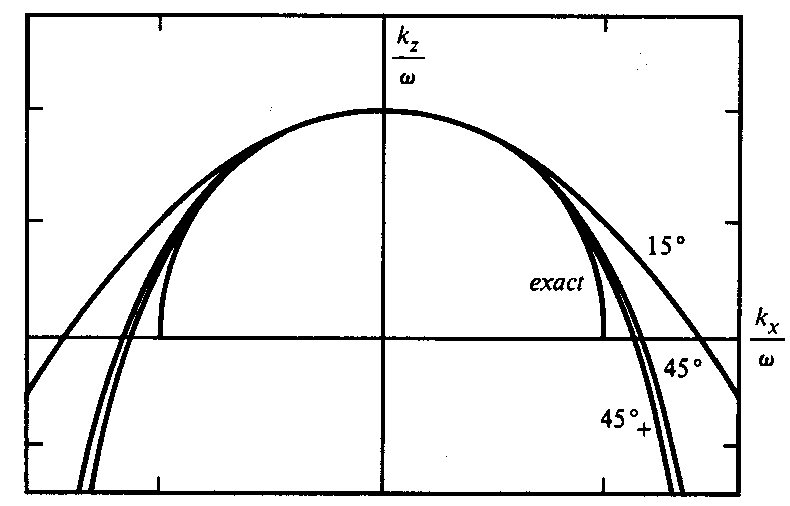
\includegraphics[width=0.6\textwidth]{omx/disper}
\caption[disper]{表\ref{tab:2.1.2}与式\ref{eq:ex2.1.6a}所示波散关系。标有$45_{+}^{\circ}$的曲线系按$R_0=cos45^{\circ}$构制,它准确地拟合于$0^{\circ}$和$45^{\circ}$的情形}
\label{fig:omx/disper}
\end{figure}
\subsection{速度随深度而变化的情形}
以算符$\partial /\partial z$代替$ik_z$可将表\ref{tab:2.1.2}的波散关系转换成表\ref{tab:2.1.3}所示偏微分方程。
\begin{table}[!ht]
\centering
\ttfamily
\small
\begin{tabularx}{\textwidth}{Y|Y}
%\begin{tabular}{p{3cm}p{4cm}p{4cm}p{5cm}}
%\toprule
\hline
$5^{\circ}$& $\frac{\partial P}{\partial z}=i[\frac{\omega}{v}]P$ \\ \hline
$15^{\circ}$& $\frac{\partial P}{\partial z}=i[\frac{\omega}{v}-\frac{vk_x^2}{2\omega}]P$ \\ \hline
$45^{\circ}$& $\frac{\partial P}{\partial z}=i[\frac{\omega}{v}-\frac{k_x^2}{2\frac{\omega}{v}-\frac{vk_x^2}{2\omega}}]P$ \\ \hline
\end{tabularx}
%\end{tabular}

\caption{速度仅与深度有关时的外推方程}
\label{tab:2.1.3}
\end{table}
表\ref{tab:2.1.3}各偏微分方程均以某个波散关系为基础,因而到头来都是以一种恒定速度假设为
基础。所以,你不能指望在速度随深度而变化时、即$v=v(z)$时方程还能有重要的应用价值或甚至还有很大用处。它们本身是无能为力描述反射的,这正好说明了它们的实际限度。

以式\ref{eq:ex2.1.6b}或表\ref{tab:2.1.3}所示各式为基础的偏移方法均称作相移法。
\subsection{延迟频率域}
安排这样一种波动计算:消除整体平移效果从而使波显得像是“停止不动”,常常有其
方便之处,有关波动延迟的这个题目将在\ref{sec:2.6}节作更详尽的研究,其时,对速度为$\hat{v}(z)$之
假想介质内的垂直传播之波引入时移$t_0$是十分容易的事,即
\begin{equation}
t_0=\int_0^z\frac{dz}{\hat{v}(z)}
\label{eq:ex2.1.10}
\end{equation}
时间域内之时延$t_0$相应于频率$\omega$域内乘以$exp(i\omega t_0)$。因此,实际波场$P(z,\omega)$与经过时
移之波场$Q(z,\omega)$有下列关系
\begin{subequaitons}

\begin{equation}
P(z,\omega)=Q(z,\omega)exp[i\omega\int_0^z\frac{dz}{\hat{v}(z)}]
\label{eq:ex2.1.11a}
\end{equation}
(方程\ref{eq:ex2.1.11}适用于义$x$空间与$k_x$空间两种情形)。对$z$微分,得
\begin{equation*}
\frac{\partial P}{\partial z}=\frac{\partial Q}{\partial z}\exp[i\omega\int_0^z\frac{dz}{\hat{v}(z)}]
+Q(z,\omega)\frac{i\omega}{\hat{v}(z)}\exp[i\omega\int_0^z\frac{dz}{\hat{v}(z)}]
%P(z,\omega)=Q(z,\omega)exp[i\omega\int_0^z\frac{dz}{\hat{v}(z)}]
%\label{eq:ex2.1.11b}
\end{equation*}
或
\begin{equation}
\frac{\partial P}{\partial z}=exp[i\omega\int_0^z\frac{dz}{\hat{v}(z)}][\frac{\partial}{\partial z+\frac{i\omega}{\hat{v}}}]Q
\label{eq:ex2.1.11b}
\end{equation}
\label{eq:ex2.1.11}
\end{subequations}
然后,将\ref{eq:ex2.1.11}代入表\ref{tab:2.1.3},得到表\ref{tab:2.1.4}所列各种延迟方程。
\begin{table}[!ht]
\centering
\ttfamily
\small
\begin{tabularx}{\textwidth}{Y|Y}
%\begin{tabular}{p{3cm}p{4cm}p{4cm}p{5cm}}
%\toprule
\hline
$5^{\circ}$& $\frac{\partial Q}{\partial z}=0                +i\omega[\frac{1}{v}-\frac{1}{\hat{v}}]Q$ \\ \hline
$15^{\circ}$& $\frac{\partial Q}{\partial z}=-i\frac{vk_x^2}{2\omega}Q      +i\omega[\frac{1}{v}-\frac{1}{\hat{v}}]Q$ \\ \hline
$45^{\circ}$& $\frac{\partial P}{\partial z}=-i\frac{\frac{k_x^2}}{{2\frac{\omega}{v}-\frac{vk_x^2}{2\omega}}}       +i\omega[\frac{1}{v}-\frac{1}{\hat{v}}]Q$ \\ \hline
\end{tabularx}
%\end{tabular}

\caption{相移方程的延迟形式}
\label{tab:2.1.4}
\end{table}
\subsection{横向速度变化}
因平方根已用多项式比值近似,表\ref{tab:2.1.3}或表\ref{tab:2.1.4}各式只须利用$(ik_x)^2=\partial^2/\partial x^2$
关系就可从水平波数域L反变换至水平空间域$x$。与前相同,所得结果对很宽范围的速度关系$v=v(x,z)$
均成立,即使看来似乎导数不允许这样做。通常将选择$\hat{v}(z)$
为$v(x,z)$的某种类
型之水平方向平均值,不过,允许$\hat{v}$成为一个$x$的函数将产生许多新项,它们很难处理,而忽
略它们又会引起一些潜在的危险,所以,一般是使$\hat{v}$与$z$有关而与$x$无关。
\subsection{分离法}
对表\ref{tab:2.1.3}与表\ref{tab:2.1.4}中各方程的空间$x$域的形式习惯上是采用分离法求其数值解,那就
是说,每推进一微小的$\Delta z$步长就要交替利用下列两种外推算子
\begin{subequaitons}

\begin{equation}
P(z,\omega)=Q(z,\omega)exp[i\omega\int_0^z\frac{dz}{\hat{v}(z)}]
\label{eq:ex2.1.11a}
\end{equation}

\begin{equation}


\end{equation}
\label{eq:ex2.1.11}
\end{subequations}